\documentclass[11pt,a4paper]{ltjsarticle}
\usepackage{amsmath,amssymb}
\usepackage{graphicx}
\usepackage{booktabs}
\usepackage{array}
\usepackage{url}
\usepackage{luatexja-fontspec}
\setmainjfont{HaranoAjiMincho-Regular}
\setsansjfont{HaranoAjiGothic-Medium}
\linespread{1.05}\selectfont

% Recommended PDF filename:
% 2611193_HeizoNakai_visual_media_processing1_dai5kai.pdf
% Example build command:
% latexmk -g -lualatex -jobname=2611193_HeizoNakai_visual_media_processing1_dai5kai main.tex

\begin{document}

\begin{center}
{\LARGE \textbf{視覚メディア処理I 第5回レポート}}
\end{center}
\vspace{1em}

\begin{flushright}
提出日: \today \\
学籍番号: 2611193 \\
氏名: 中井 平蔵
\end{flushright}

\section*{ORBによる局所特徴記述}

本レポートでは、ORB（Oriented FAST and Rotated BRIEF）について説明する。
ORBは、特徴点検出手法であるFASTと、バイナリ特徴記述手法であるBRIEFを組み合わせ、さらに回転に対する頑健性を加えた手法である。
SIFTやSURFと比較して計算量とメモリ使用量が小さく、リアルタイム処理に適していることが大きな特徴である。

ORBの処理は、主に特徴点検出、方向推定、特徴記述から構成される。

\subsection*{1. 特徴点検出}

最初に、FASTを用いて画像中の特徴点を検出する。
FASTでは、注目画素を中心とする半径3画素の円周上に配置された16画素を調べる。

\begin{figure}[htbp]
\centering
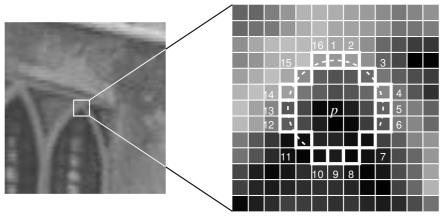
\includegraphics[width=0.94\linewidth]{fast_speedtest.jpg}
\caption{FASTで注目画素の周囲半径3画素の16画素を調べる様子}
\label{fig:fast-fast}
\end{figure}

図の出典: 鳥取大学 OpenCV-Python Tutorials 1 documentation「コーナー検出のためのFASTアルゴリズム」,
\url{https://labs.eecs.tottori-u.ac.jp/sd/Member/oyamada/OpenCV/html/py_tutorials/py_feature2d/py_fast/py_fast.html}
（閲覧日: 2026年6月23日）。

FASTの判定では、注目画素の明るさを $I_p$、円周上の各画素の明るさを $I_{x}$ とする。
ここで、$p$ は注目画素の位置、$x$ は注目画素の周囲16画素のうちの任意の1画素を表す。
しきい値を $t>0$ とすると、各画素は次の3値で表せる。

\begin{equation}
s(x)=
\begin{cases}
1 & I_x \geq I_p + t \\
-1 & I_x \leq I_p - t \\
0 & \text{それ以外}
\end{cases}
\label{eq:fast-state}
\end{equation}

このとき、円周上の連続する $n$ 画素がすべて明るい側または暗い側のしきい値を超えれば、注目画素をコーナー候補と判定する。
ここで、$n$ は連続して条件を満たす画素数、$k$ は連続区間の始点を表す。
式で書くと、

\begin{equation}
\exists k \in \{1,\dots,16\}\ \text{such that}\ \sum_{j=0}^{n-1}\lvert s(x_{k+j})\rvert = n
\label{eq:fast-contiguous}
\end{equation}

である。
ORBでは一般にFAST-12を用い、円周上の16画素のうち、連続する12画素が注目画素より十分に明るい、または暗い場合にコーナーと判定する。
画素値の比較だけで済むため、画像微分などを用いる特徴点検出手法よりも高速に計算できる。
ただし、検出された各点が、画像の変化に対してどの程度安定して検出できるかまでは十分に評価できない。
そこでORBでは、Harrisコーナー応答を用いて各特徴点のコーナーらしさを数値化し、その値が大きい点を優先的に選択する。
Harrisコーナー応答とは、特徴点の周囲における縦方向と横方向の輝度変化を調べ、両方向で変化が大きい点ほど、明確なコーナーであると評価する指標である。

また、ORBでは、元画像を段階的に縮小した画像ピラミッドを作成し、各解像度の画像に対して特徴点検出を行う。
FASTは一定の画素範囲を用いてコーナーを検出するため、物体の見かけの大きさが変化すると、同じ特徴点を検出できない場合がある。
しかし、複数の解像度で検出を行うことで、大きく写った特徴は縮小画像上で、小さく写った特徴は高解像度画像上で捉えられるため、ORBはある程度のスケール変化に対応できる。

\subsection*{2. 方向推定}

次に、検出した特徴点ごとに方向を推定する。
ここで推定するのは、特徴点周辺の画素分布に対する主方向である。
通常のFASTは特徴点の位置のみを検出するため、画像が回転すると同じ特徴点でも異なる特徴記述子が生成されることがある。
ORBでは、特徴点周辺の画素の輝度値を質量とみなし、その重心を求める強度重心法を使用する。
画像モーメントを

\begin{equation}
m_{pq}=\sum_{x,y} x^p y^q I(x,y)
\label{eq:moment}
\end{equation}

ここで、各記号は次の意味を表す。
\begin{itemize}
\item $m_{pq}$: 画像モーメント
\item $I(x,y)$: 座標 $(x,y)$ の画素の輝度値
\item $x,y$: 特徴点を中心とした相対座標
\item $p,q$: モーメントの次数
\end{itemize}
特に $m_{10}$ は $x$ 方向の重み付き和、$m_{01}$ は $y$ 方向の重み付き和を表す。
これらから、特徴点の主方向角 $\Theta$ は以下の式で求める。

\begin{equation}
\Theta=\operatorname{atan2}(m_{01},m_{10})
\label{eq:orientation}
\end{equation}

ここで、$\Theta$ は特徴点の主方向角であり、$\operatorname{atan2}$ は $m_{01}$ と $m_{10}$ の符号を考慮して角度を求める関数である。
これは、特徴点の中心から輝度分布の重心へ向かう方向を、その特徴点の主方向とする方法である。

\subsection*{3. 特徴記述}

特徴記述とは、特徴点の周囲の局所的な見え方を数値列として表現する処理である。
最後に、Rotated BRIEFを用いて特徴記述子を生成する。
BRIEFでは、特徴点周辺に複数の画素対を設定し、それぞれの輝度値を比較する。
ここで、$p_i'$ と $q_i'$ は比較対象となる2つの画素位置であり、$I(p_i')$ と $I(q_i')$ はそれぞれの輝度値である。
この比較結果を1ビットに変換したものを用いる。
各ビットは、特徴点周辺の局所的な明暗関係を表している。
各ビットは

\begin{equation}
\tau_i=
\begin{cases}
1 & I(p_i')<I(q_i') \\
0 & I(p_i')\geq I(q_i')
\end{cases}
\label{eq:brief-bit}
\end{equation}

として求められる。
この比較を多数の画素対について行い、結果を0と1からなるバイナリ列として並べる。
一般的なORB記述子は256ビットであり、一つの特徴量を32バイトで表現できる。

通常のBRIEFは比較する画素位置が固定されているため、画像の回転に弱い。
そこでORBでは、先に推定した方向 $\theta$ に合わせて画素対の配置を回転させる。
これにより、画像が回転した場合でも、特徴点を基準としてほぼ同じ位置関係にある画素を比較できる。
つまり、回転前に選んだ画素対を、そのまま固定した座標系で比べるのではなく、特徴点ごとの主方向にそろえてから比較することで、向きの違いによる記述子の変化を抑えている。
また、ORBでは、比較結果の分散が大きく、互いの相関が小さい画素対を選択することで、記述子の識別性能を高めている。

\subsection*{長所}

ORBの大きな長所は、特徴記述子がバイナリ形式であることである。
SIFTなどの浮動小数点ベクトルでは、特徴量間の比較にユークリッド距離を用いる。
一方、ORBでは、異なるビットの数を数えるハミング距離を用いる。
ハミング距離はXOR演算とビットカウントによって計算できるため、CPU上で非常に高速に処理できる。
また、記述子のサイズが小さいため、メモリ使用量だけでなく、キャッシュミスやデータ転送量も削減できる。
このようにORBは、特徴点検出、特徴記述、特徴量比較の各段階で計算コストを抑えている。

さらに、ORBはFASTを基礎としているため、特徴点検出そのものも比較的軽量である。
画像ピラミッドを用いて複数の解像度で特徴点を検出できるので、完全な不変ではないものの、ある程度のスケール変化に対応できる。
そのため、限られた計算資源の中で、特徴点を高速に処理したい場面に向いている。

\subsection*{短所}

一方、ORBには、大きなスケール変化、視点変化、照明変化に対する頑健性がSIFTなどと比較して低いという短所がある。
バイナリ特徴量は局所的な画素値の大小関係に基づくため、画像の見え方が大きく変化すると、特徴記述子のビットも変化しやすい。
また、画像ピラミッドによってスケール変化に対応しているものの、スケール空間を厳密に構築するSIFTほどのスケール不変性は持たない。
そのため、撮影条件が大きく変わる場面や、同じ対象をさまざまな角度から確実に照合したい場面では、十分な性能を得にくいことがある。

\end{document}
